\begin{figure*}[htbp]
\centering
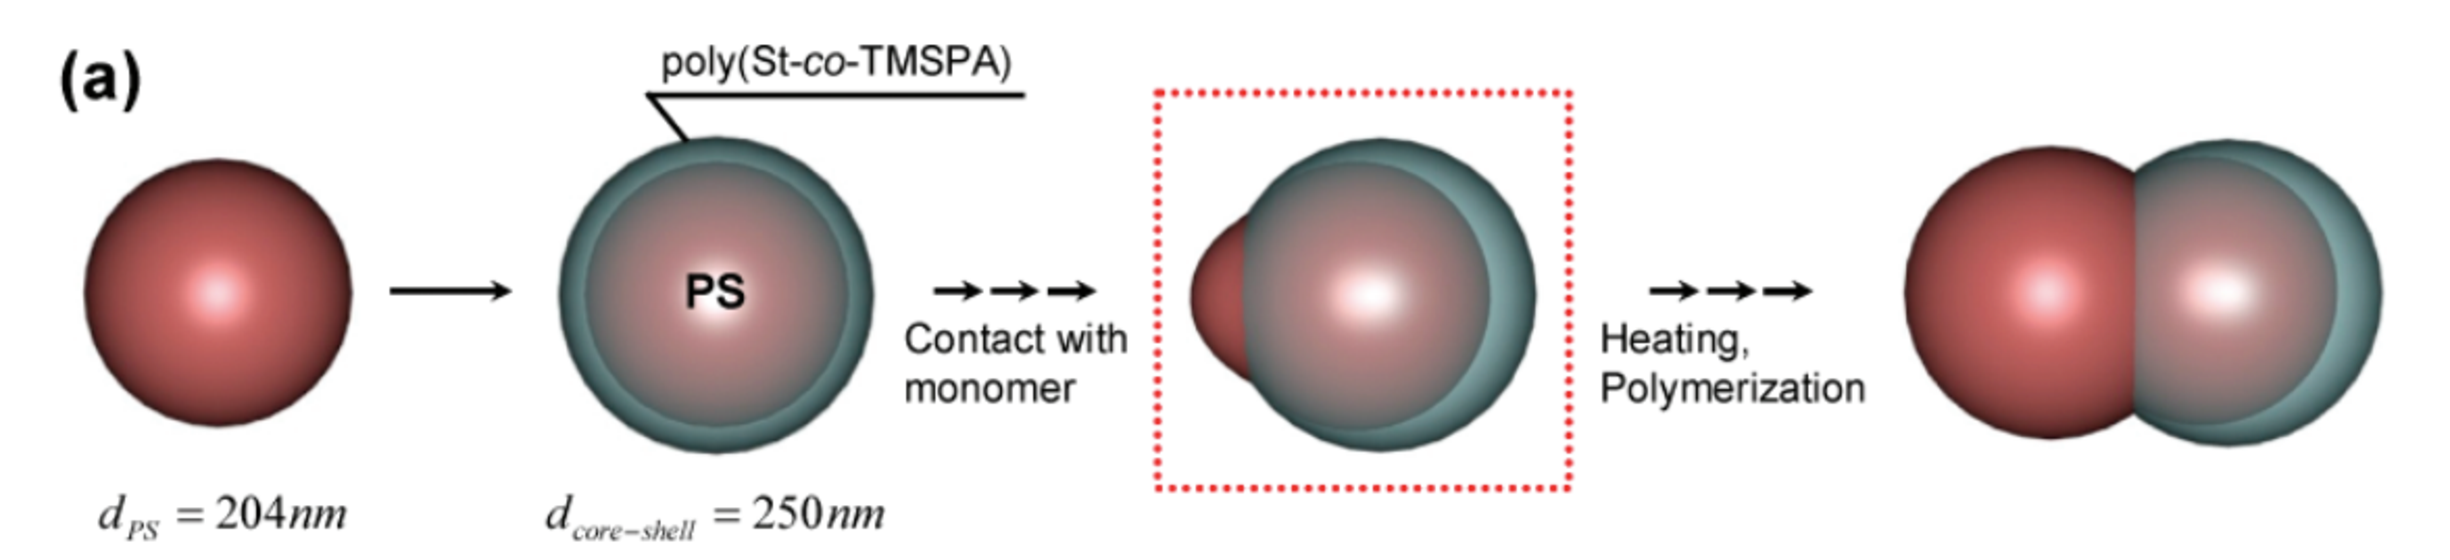
\includegraphics[width=1\textwidth]{figures/synthesisScheme.pdf}
\caption{\label{fig:synthesis-scheme}\emph{Schematic of the synthesis procedure used to make dumbbells.}
From Ref.~\cite{Park2010}}
\end{figure*}

The synthesis procedure for all the particles used in this dissertation is illustrated in Figure~\ref{fig:synthesis-scheme}.
The spherical polystyrene particles used in Chapter~\ref{chap:sphere-isotropic} correspond to the red sphere on the left of Figure~\ref{fig:synthesis-scheme}.
The polystyrene spheres are then swollen with a mixture of styrene and TMSPA monomers.
After polymerizing the new monomer, we have the spherical core-shell poly(sty-co-TMSPA) particles that are illustrated in the second step of Figure~\ref{fig:synthesis-scheme}.
Adding and polymerizing new monomer a second time does not result in larger spheres, instead, the newly polymerized material forms a second lobe and we have the dumbbell particles used in Chapter~\ref{chap:dumbbell-crystal} and illustrated in the final step of Figure~\ref{fig:synthesis-scheme}.



\section{Polystyrene Sulfonate Spheres}
\label{chap:synthesis:ps}

The synthesis of polystyrene-sulfonate spheres begins with the assembly of a 500 mL three-neck round-bottom flask fitted with a cold-water reflux condenser, teflon blade stirrer, and a nitrogen inlet. 
The assembled reaction vessel is lowered into a temperature controlled water bath set to 65$^\circ$ C.
While waiting for the bath to come up to temperature, the reagents are prepared.
First, methanol and DI water in the quantities indicated in Figure~\ref{fig:sphere-synthesis:recipe} are combined in a 250 mL glass bottle.
Second, the indicated quantity of ionic co-monomer, 4-vinylbenzenesulfonate (VBS), is added to the methanol/DI solution and shaken to dissolve.
Third, the appropriate amount of water-soluble initiator, potassium persulfate (KPS), is added to the methanol/DI/VBS solution and shaken to dissolve, which for KPS can take a few minutes.
Fourth, the styrene monomer is pipetted from the stock bottle into a 40 mL glass vial.
Once the water bath temperature reaches 65$^\circ$ C and the KPS has completely dissolved, the methanol/DI/VBS/KPS solution is poured into the reaction vessel, the stirring speed is set to ~400 RPM, and the atmosphere in the vessel is purged with a quick burst of nitrogen.
In practice, the stir speed should be as fast as possible without causing the liquid to splash into the connecting joints of the flask.
Adding the room temperature solution to the reaction vessel will cause the temperature to  drop.
Once the water bath temperature has recovered, the styrene monomer is poured into the reaction vessel and the nitrogen is set to slowly flow through the vessel as the polymerization reaction proceeds for at least eight hours, although longer reaction times will result in more complete conversion of monomer into polymer.

Figure~\ref{fig:sphere-synthesis:SEM} shows an SEM image of the spheres produced by using the quantities of reagents listed in Figure~\ref{fig:sphere-synthesis:recipe}.

There are a multiple ways to change the final size of particles synthesized with this technique including changing the quantity of VBS, the quantity of styrene, or the quantity of methanol \cite{CHONDE:1981p1047}.
The different size spheres used in Chapter~\ref{chap:sphere-isotropic} are made by varying the amount of methanol in the reaction while keeping the combined volume of DI water and methanol constant.
As described in Ref.~\cite{CHONDE:1981p1047}, increasing the fraction of methanol results in larger diameter spheres if the quantities of all the other reagents are fixed.

It should be noted that the final composition of spheres made with the formulation in Figure~\ref{fig:sphere-synthesis:recipe} is not the only possible formulation.
Methacrylic acid and divinylbenzene have both been successfully incorporated with styrene using this procedure.
When methacrylic acid is included, typically in quantities up to 10\% of the total monomer, the resulting polymer is a random co-polymer of styrene and methacrylic acid with carboxylic acid groups present on the surface of the spheres.
These carboxylic acid groups can then be used to covalently attach other species.
For example, proteins are frequently attached to particles presenting carboxylic acid via carbodiimide chemistry.
When divinylbenzene is included in the monomer mixture, typically in quantities up to a few percent of the total monomer, the resulting polymer network is no longer composed of linear polymer chains but is composed of polymer chains which are covalently cross-linked.
Cross-linking particles have a very different physical character than linear polymer particles and are desirable for many uses because of their limited ability to swell \cite{Sheu:1990}.

\begin{figure*}[htbp]
\centering
	\subfloat[Details of the synthesis of polystyrene sulphonate spheres.]{
	\label{fig:sphere-synthesis:recipe}
	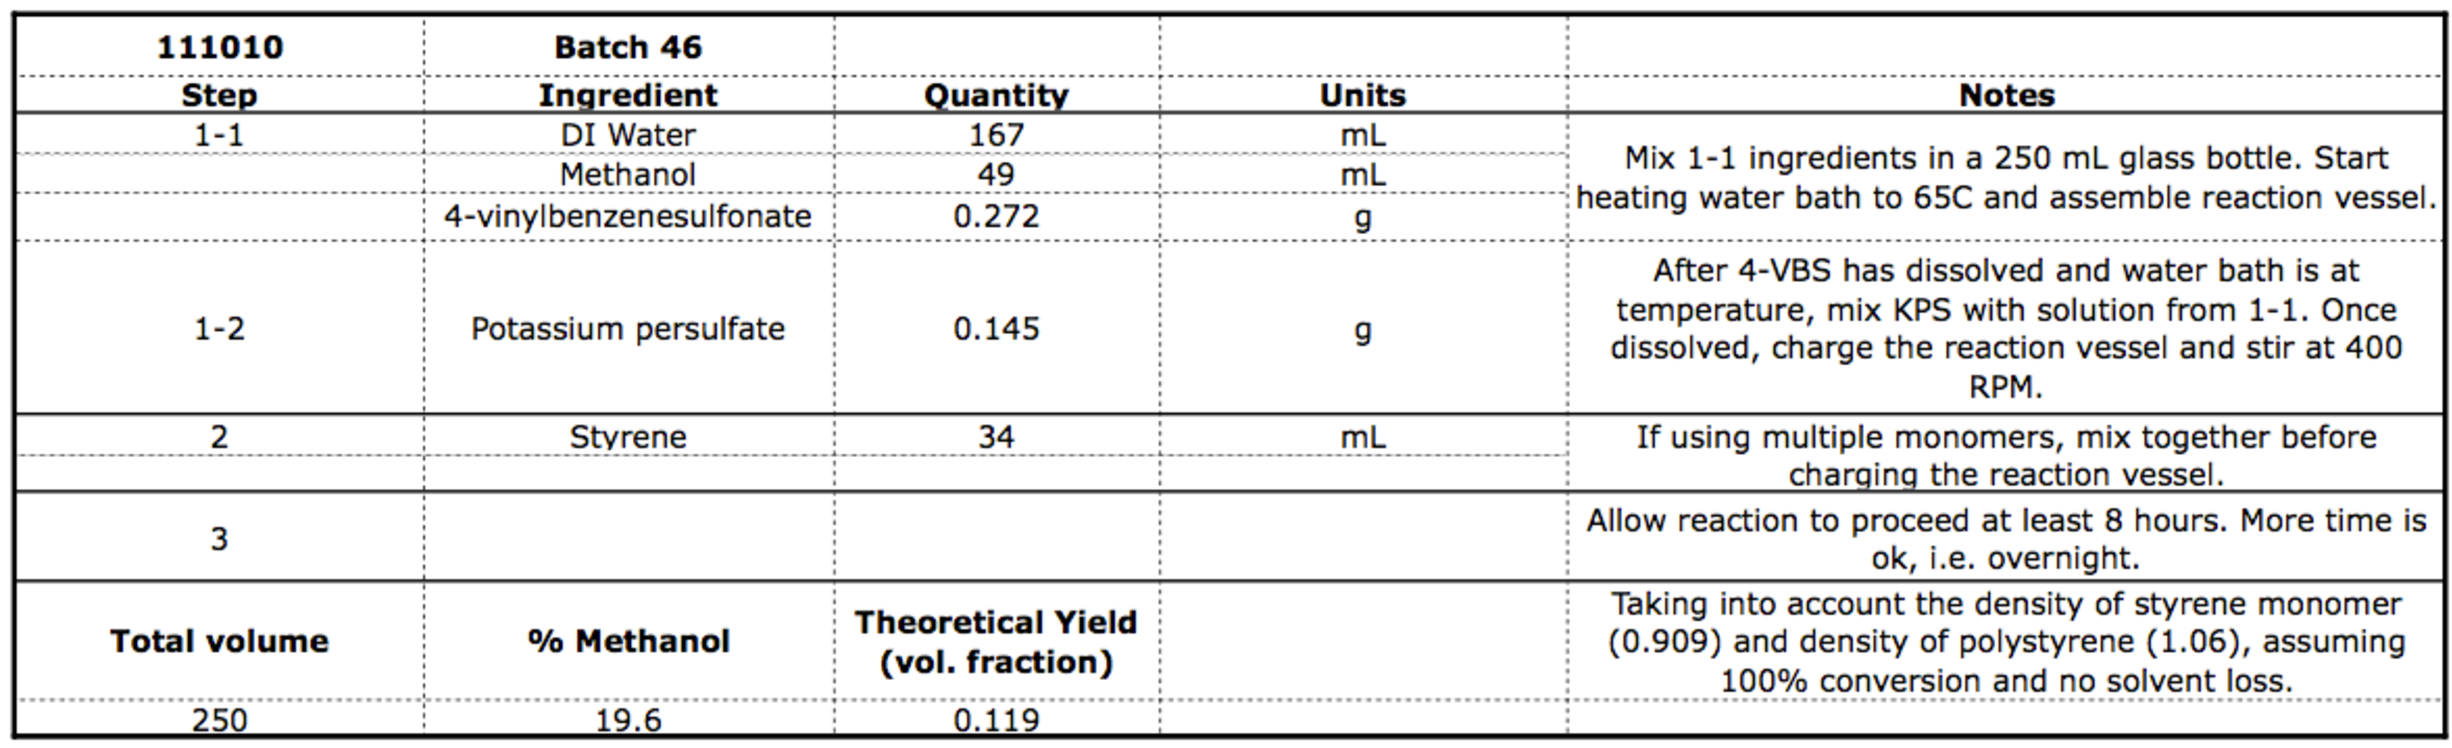
\includegraphics[width=1.0\textwidth]{figures/PSSphereRecipe.pdf}
	}\\
	\subfloat[SEM image of the polystyrene spheres resulting from the recipe detailed in Figure~\ref{fig:sphere-synthesis:recipe}.]{
	\label{fig:sphere-synthesis:SEM}
	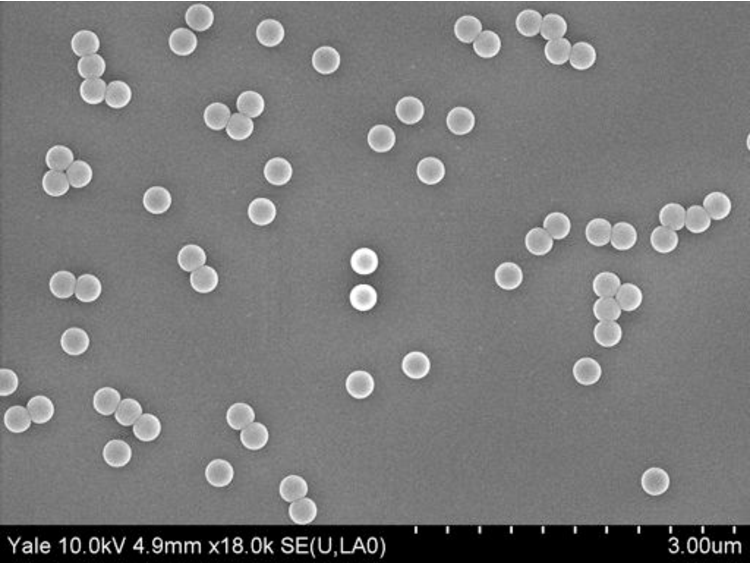
\includegraphics[width=1.0\textwidth]{figures/Batch46SEM.pdf}
	}
\caption{\label{fig:sphere-synthesis}\emph{Polystyrene sulfonate sphere synthesis.}}
\end{figure*}


\section{Poly(styrene-co-TMSPA) Core-Shell Spheres}
\label{chap:synthesis:cs}

Polystyrene spheres as synthesized by the procedure in the previous section are the starting material for the synthesis of core-shell poly(styrene-co-TMSPA) spheres.
Figure~\ref{fig:core-shell-synthesis:recipe} contains the information for four identical batches of core-shell particles that are synthesized simultaneously in separate reaction vials.
In general, though, each reaction vial can contain a different composition.
The core-shell particles used to make the dumbbells used in Chapter~\ref{chap:dumbbell-crystal} are prepared as follows, using the recipe shown in Figure~\ref{fig:core-shell-synthesis:recipe}.
First, a temperature controlled water bath is set to 70$^\circ$ C.
Second, 15 mL of as-synthesized polystyrene sulfonate spheres are combined with 12 mL of DI water in a 40 mL glass vial.
Third, 9.9 mg of oil-soluble initiator,  azobisisobutyronitrile (AIBN), is weighed into a 20 mL glass vial.
Fourth, 1.78 mL of styrene monomer and 0.20 mL of TMSPA are added to the vial containing AIBN and shaken to dissolve.
Once the AIBN has dissolved, 1.79 mL of the monomer mixture is added to the 40 mL vial containing the polystyrene sphere suspension.
The 40 mL vial is then closed, sealed with teflon tape and mixed by vortexing for one minute.
This procedure is repeated if more than one core-shell synthesis is being done simultaneously.
The reaction vials are then loaded into a plastic bottle which has been fixed to a metal stirring shaft.
The entire assembly is attached to a mixer and submerged in the 70$^\circ$ water bath while rotating at approximately 300 RPM.
The polymerization reaction is allowed to proceed for at least eight hours, but longer reaction times will result in more complete conversion of monomer to polymer.

Figure~\ref{fig:core-shell-synthesis:SEM} shows an SEM image of the core-shell spheres produced by using the quantities of reagents listed in the first column of Figure~\ref{fig:core-shell-synthesis:recipe}.

The surface of the core-shell spheres is composed of a random co-polymer of styrene and TMSPA.
As discussed in Chapter~\ref{chap:conclusions}, the TMSPA is not only necessary for the production of dumbbells, it also allows for the covalent attachment of other chemical species via silane chemistry which can significantly alter the nature of the surface \cite{DerVoort:1996}.

\begin{figure*}[htbp]
\centering
	\subfloat[Details of the synthesis of poly(styrene-co-TMSPA) core-shell spheres.]{
	\label{fig:core-shell-synthesis:recipe}
	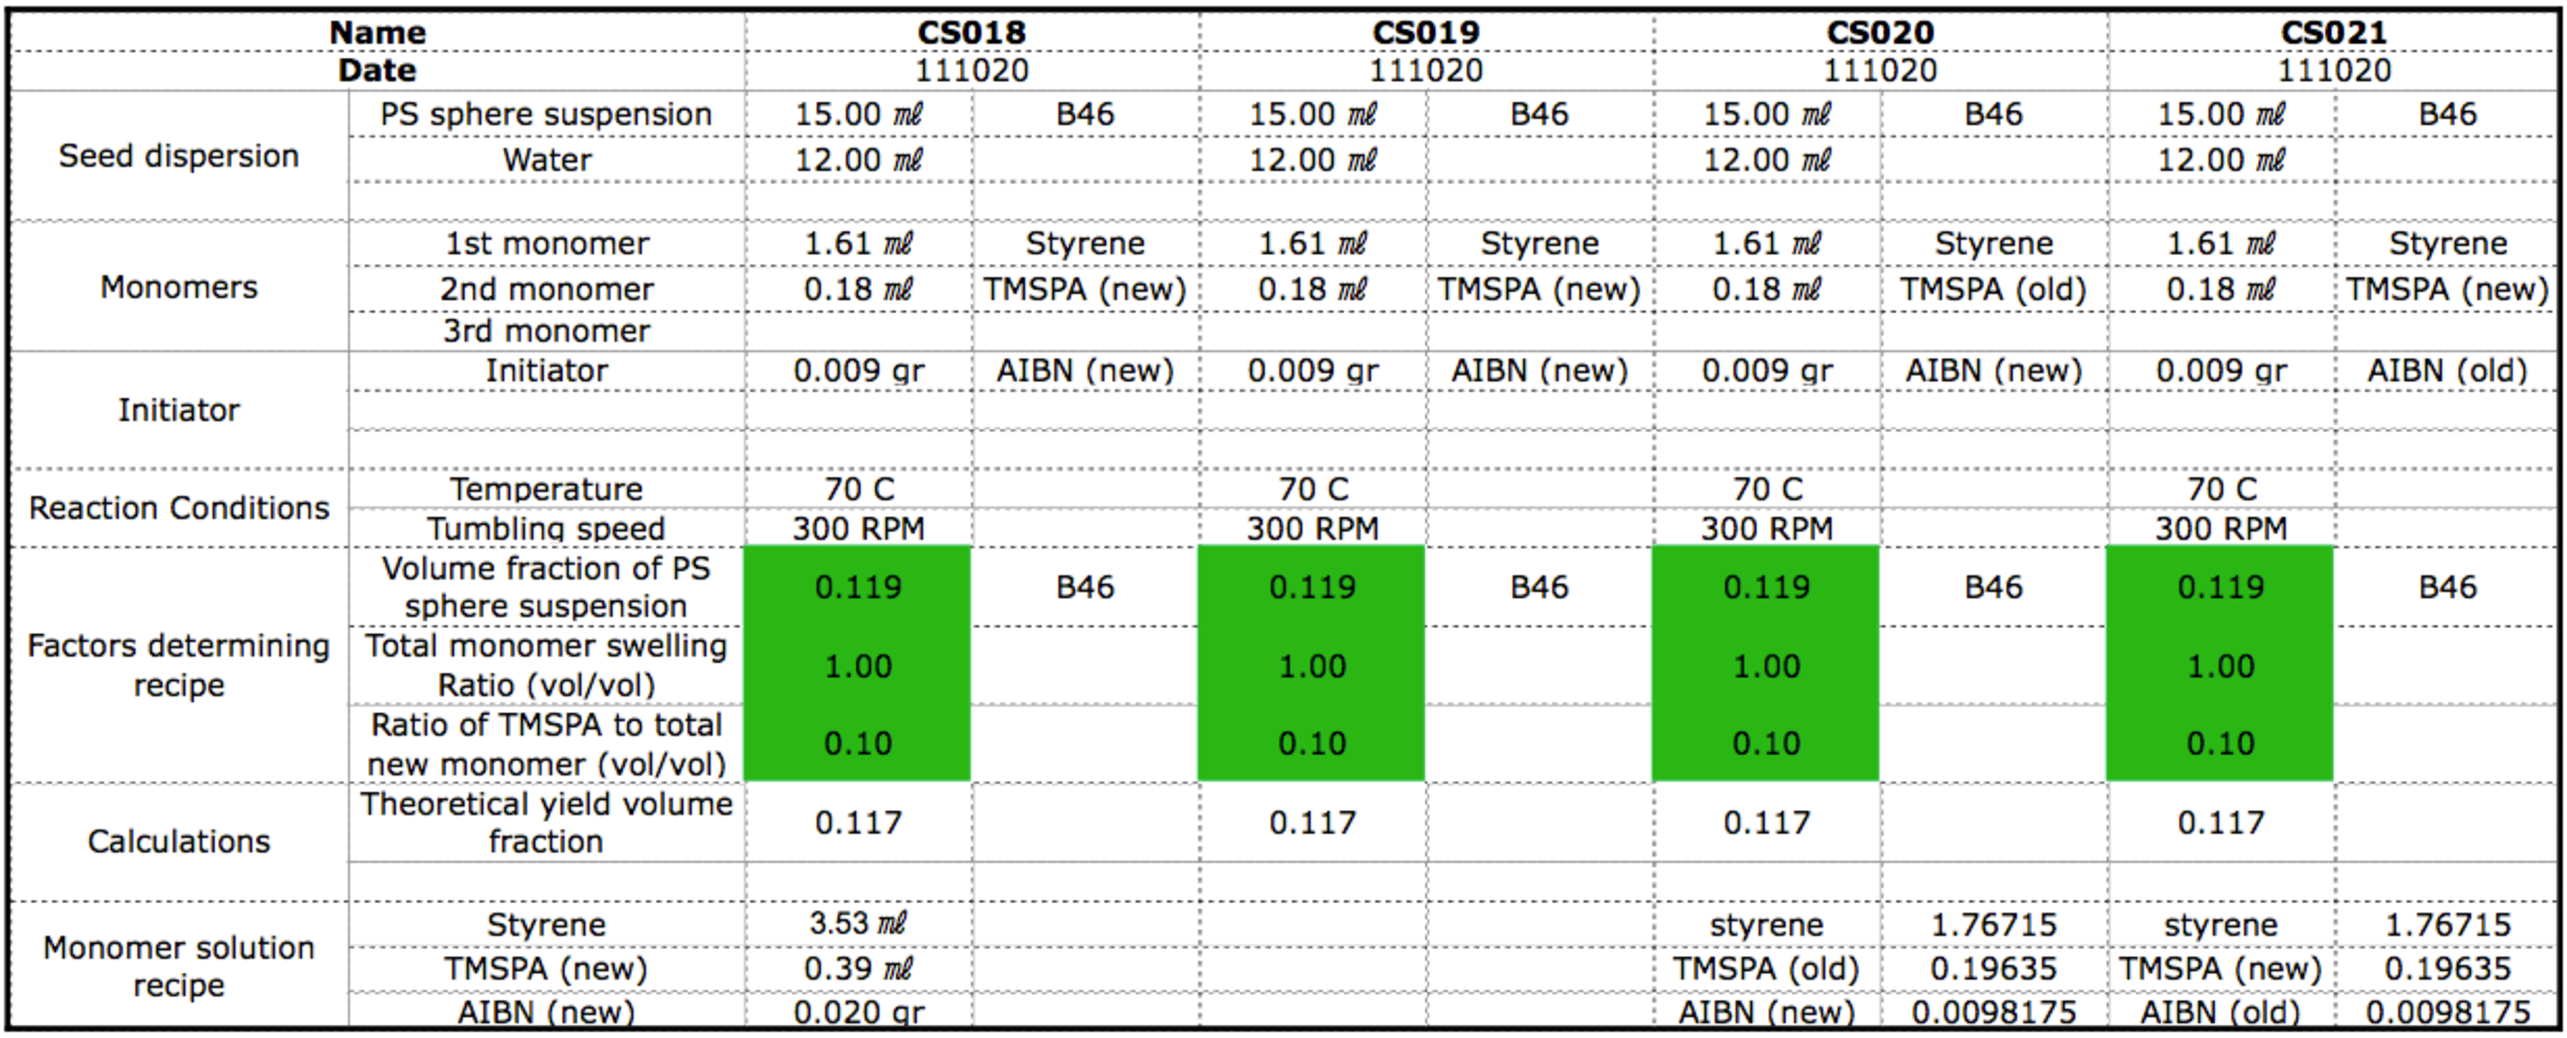
\includegraphics[width=1.0\textwidth]{figures/CoreShellSphereRecipe.pdf}
	}\\
	\subfloat[SEM image of the poly(styrene-co-TMSPA) core-shell spheres resulting from the recipe detailed in the first column of Figure~\ref{fig:core-shell-synthesis:recipe} (CS018).]{
	\label{fig:core-shell-synthesis:SEM}
	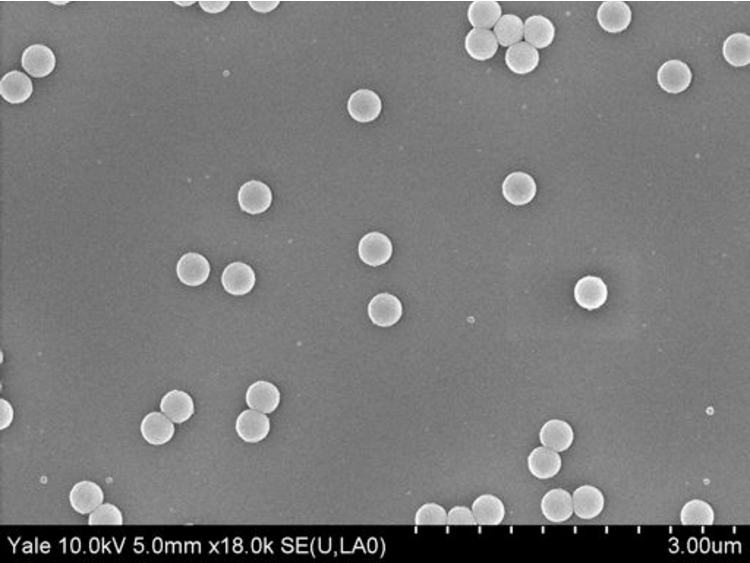
\includegraphics[width=1.0\textwidth]{figures/CS018.pdf}
	}
\caption{\label{fig:core-shell-synthesis}\emph{Poly(Styrene-co-TMSPA) core-shell sphere synthesis.}}
\end{figure*}


\section{Dumbbells}
\label{chap:synthesis:db}

Core-shell spheres as synthesized by the procedure in the previous section are the starting material for the synthesis of dumbbells.
Figure~\ref{fig:dumbbell-synthesis:recipe} contains the information for four batches of dumbbell particles that are synthesized simultaneously in separate reaction vials.
In general, each reaction vial can contain a different composition.
The dumbbells used in Chapter~\ref{chap:dumbbell-crystal} are prepared as follows, using the recipe shown in Figure~\ref{fig:dumbbell-synthesis:recipe}.
First, a temperature controlled water bath is set to 70$^\circ$ C.
Second, 7 mg of VBS is dissolved in 8 mL of DI water and added to the core-shell suspension.
Third, 8 mL of as-synthesized poly(styrene-co-TMSPA) spheres are combined with 3.5 mL of DI water and 1 mL of 1\% (w/w) Pluronic F108 in DI water in a 40 mL glass vial.
Fourth, 5.5 mg of oil-soluble initiator,  azobisisobutyronitrile (AIBN), is weighed into a 20 mL glass vial.
Fifth, 1.03 mL of styrene monomer is added to the vial containing AIBN and shaken to dissolve.
Once the AIBN has dissolved, 0.94 mL of the monomer mixture is added to the 40 mL vial containing the core-shell sphere suspension.
The 40 mL vial is then closed, sealed with teflon tape and mixed by vortexing for one minute.
This procedure is repeated if more than one dumbbell synthesis is being done simultaneously.
The reaction vials are then loaded into a plastic bottle which has been fixed to a metal stirring shaft.
The entire assembly is attached to a mixer and submerged in the 70$^\circ$ water bath while rotating at approximately 300 RPM.
The polymerization reaction is allowed to proceed for at least eight hours, but longer reaction times will result in more complete conversion of monomer to polymer.

Figure~\ref{fig:dumbbell-synthesis:SEM} shows an SEM image of the dumbbells produced by using the quantities of reagents listed in the first column of Figure~\ref{fig:dumbbell-synthesis:recipe}.
Figure~\ref{fig:jDB09-detail} shows a high-magnification SEM image of the same dumbbells shown in Figure~\ref{fig:dumbbell-synthesis:SEM} and highlights the difference in roughness between the poly(Styrene-co-TMSPA) lobe and the newly-formed polystyrene lobe.

This procedure for making dumbbells can be modified to produce particles with varying aspect ratios and surface chemistries.
The simplest way to vary the aspect ratio of a batch of dumbbells is to change the quantity of new monomer added.
In the recipe highlighted here, the volume of new monomer is such that the new lobe of each dumbbell will be the same size as the core-shell seed particle.
Adding more or less monomer will result in a larger or smaller new lobe, as demonstrated in Ref.~\cite{Park2010}.
The surface chemistry of the new lobe depends on the composition of added monomer and we have successfully synthesized dumbbells with isotropic surface chemistry by including TMSPA to the monomer mixture in this step.
These isotropic dumbbells were used in the demonstration of dumbbell behavior at an oil/water interface in Chapter~\ref{chap:conclusions}.
Other monomers, such as methacrylic acid, can be included in the monomer mixture to provide enhanced chemical functionality.

\begin{figure*}[htbp]
\centering
	\subfloat[Details of the synthesis of dumbbells.]{
	\label{fig:dumbbell-synthesis:recipe}
	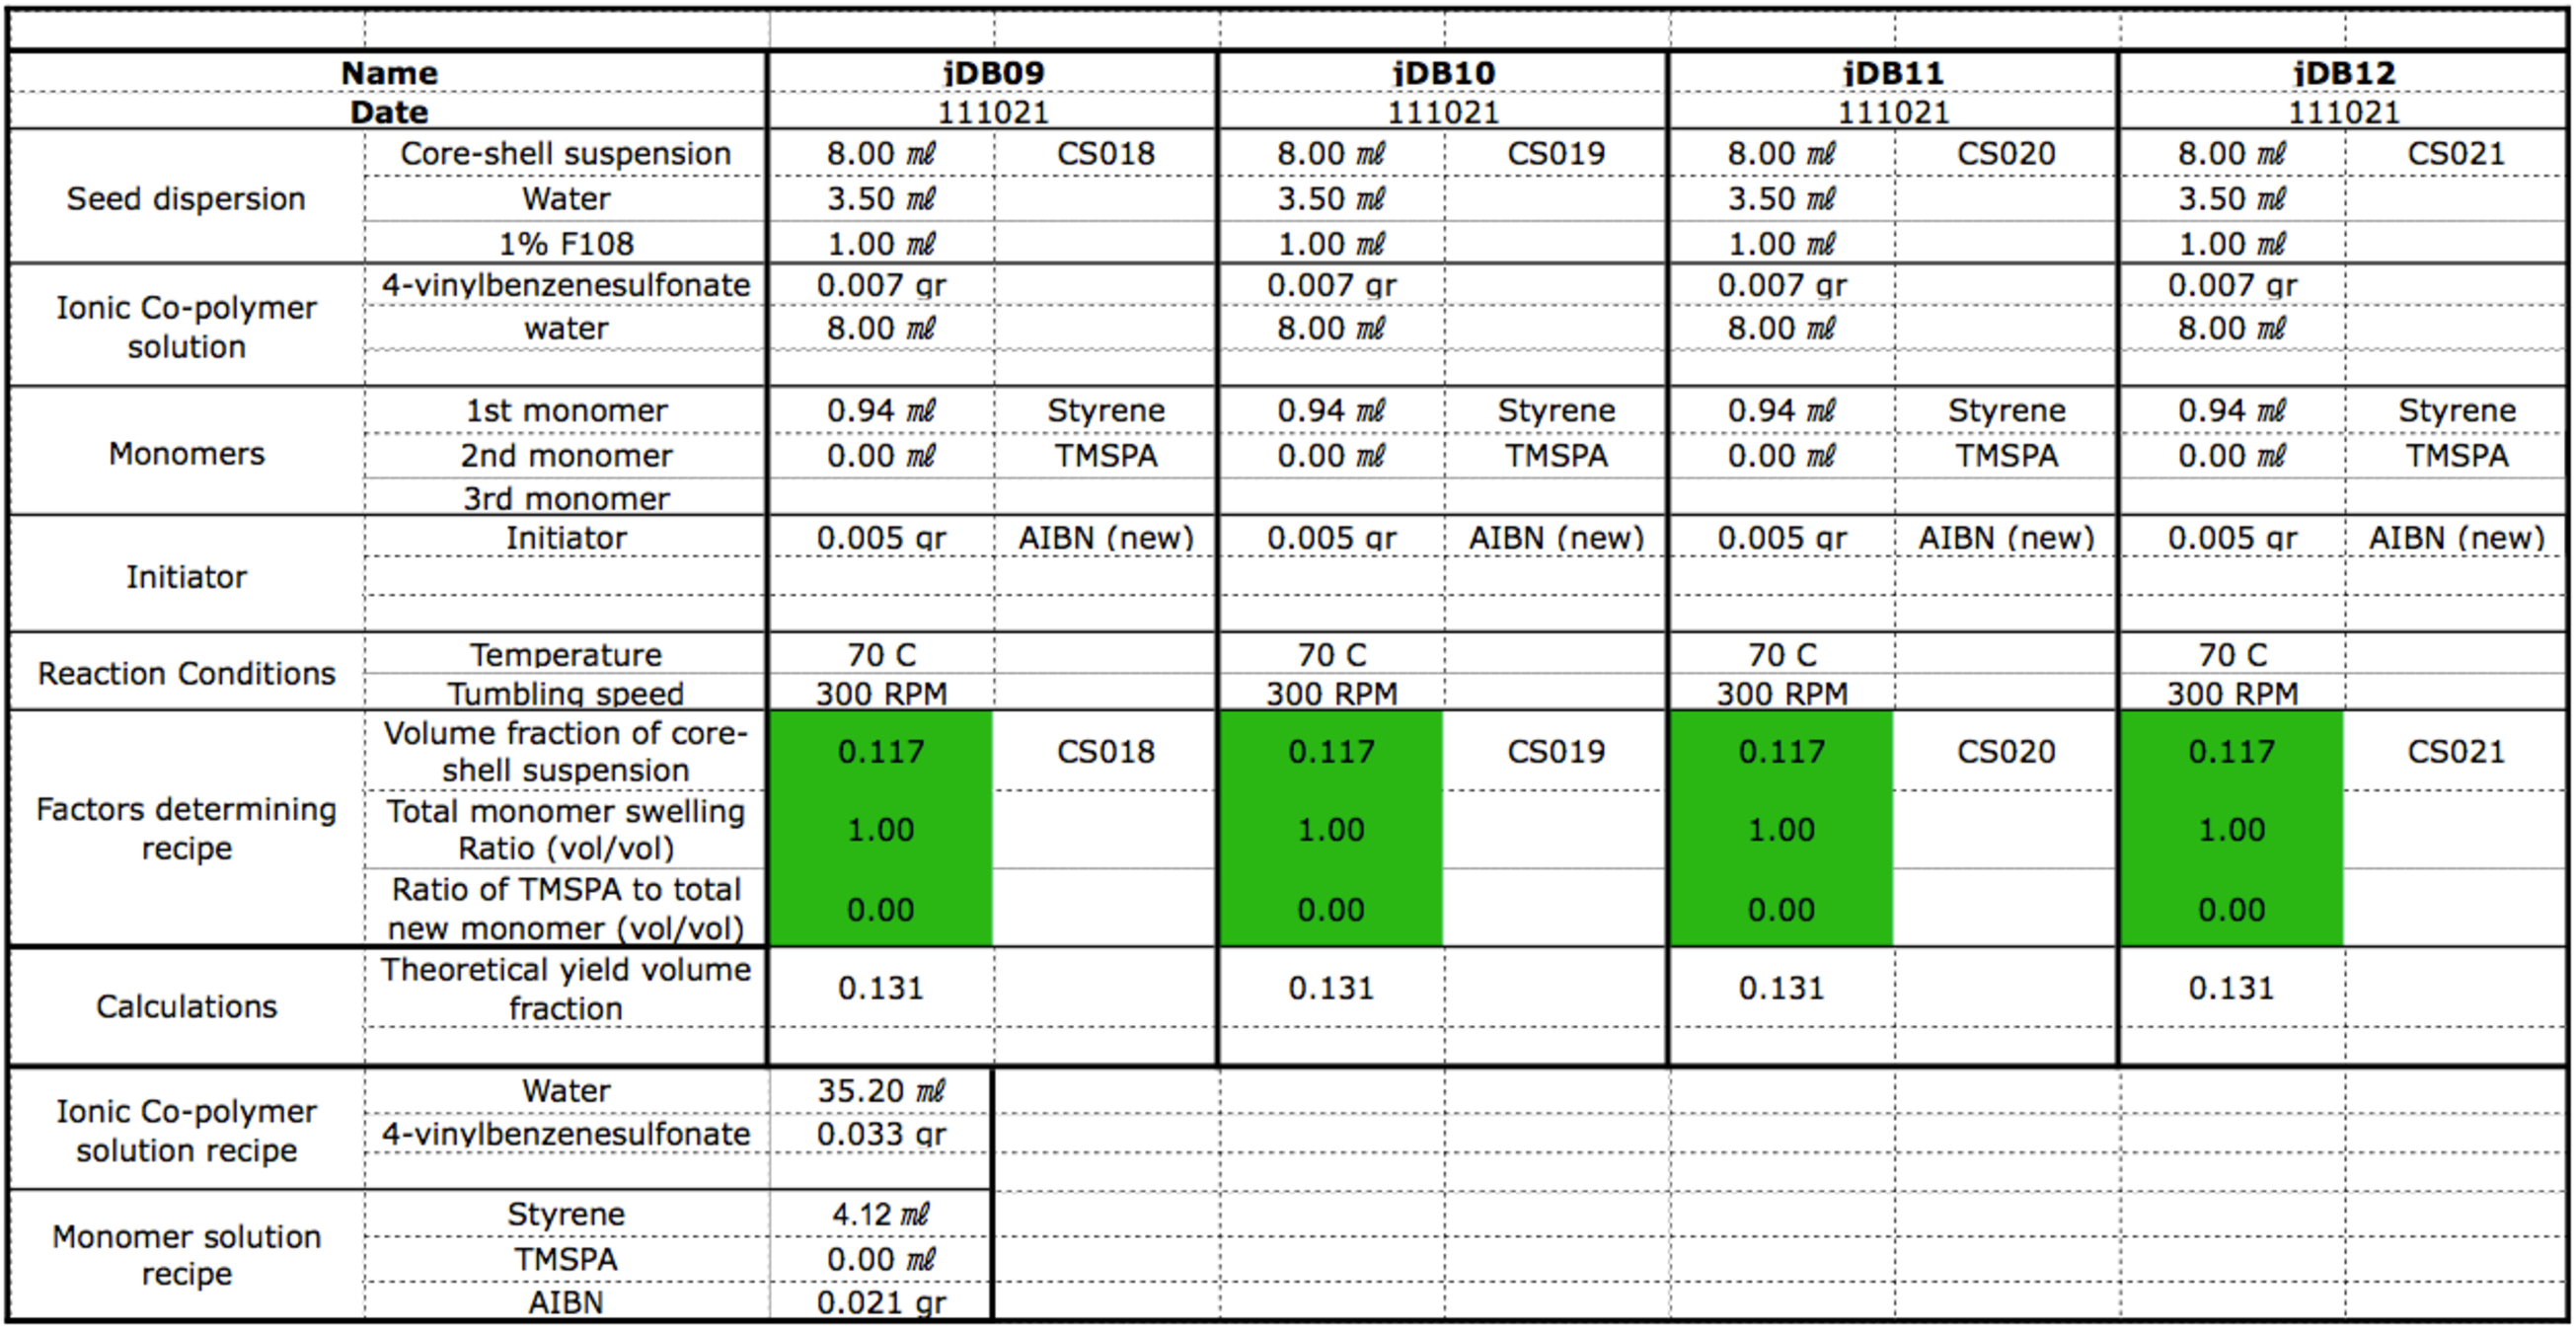
\includegraphics[width=1.0\textwidth]{figures/DumbbellRecipe.pdf}
	}\\
	\subfloat[SEM image of the dumbbells resulting from the recipe detailed in the first column of Figure~\ref{fig:dumbbell-synthesis:recipe} (jDB09).]{
	\label{fig:dumbbell-synthesis:SEM}
	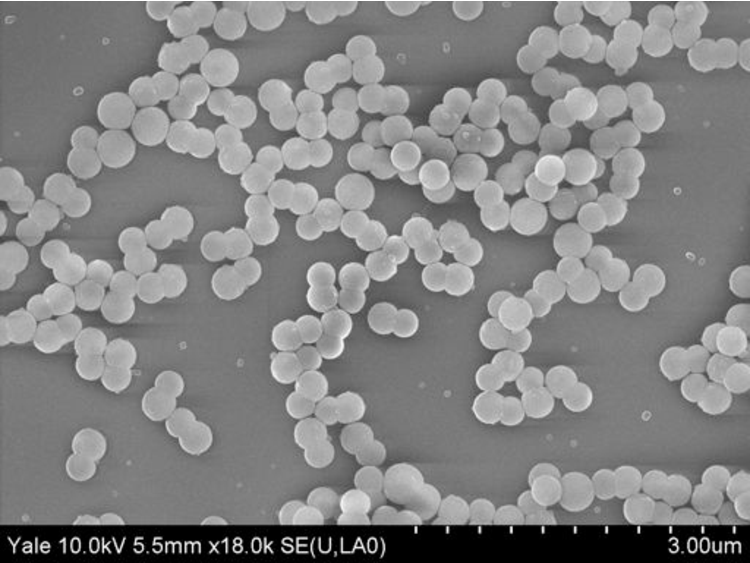
\includegraphics[width=1.0\textwidth]{figures/jDB09SEM.pdf}
	}
\caption{\label{fig:dumbbell-synthesis}\emph{Dumbbell synthesis.}}
\end{figure*}


\begin{figure*}[htbp]
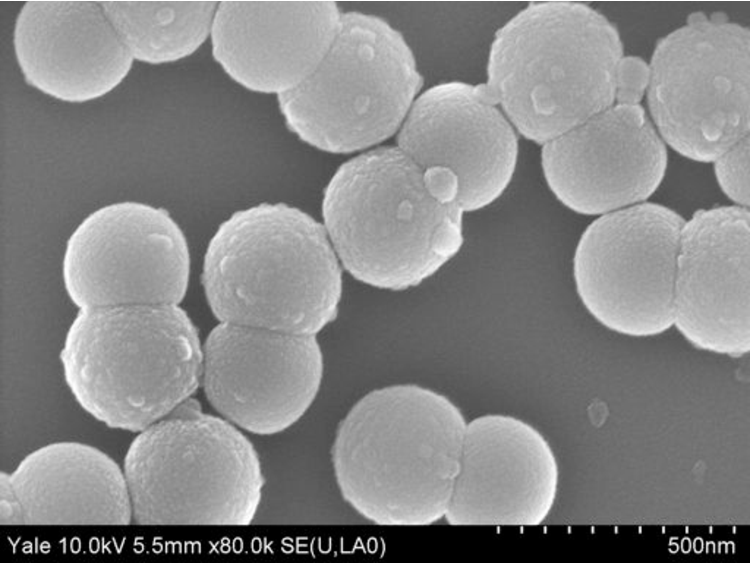
\includegraphics[width=1.0\textwidth]{figures/jDB09SEMDetail.pdf}
\caption{\label{fig:jDB09-detail} \emph{High-magnification SEM image of dumbbells.}
	High-magnification SEM image of the same dumbbells in Figure~\ref{fig:dumbbell-synthesis:SEM}. Note that the two lobes have differing degrees of roughness. The smoother lobe is primarily polystyrene and the rougher lobe is poly(styrene-co-TMSPA).}
\end{figure*}

